
\subsection{Degree Distribution and Power Law}
% BEGIN: degree distribution and power law

% END: degree distribution and power law

\subsection{Most Important Symptoms/Diseases (4 Classes)}
% BEGIN: most important symptoms/diseases (4 classes)

% END: most important symptoms/diseases (4 classes)

\subsection{Betweenness Centrality}
% BEGIN: betweenness centrality
As shown in Figure \ref{fig:bet_entire}, the betweenness centrality of the nodes in the network follows a Power Law Distribution. This suggests
a scale-free structure of the network, with a few central nodes working as connecting actors, while the majority of the nodes have a low betweenness centrality.
Dividing the centrality values into the two classes of symptoms and diseases (Figures \ref{fig:bet_diseases} and \ref{fig:bet_symptoms}), we can see that 
the symptoms have a higher betweenness centrality than the diseases. To understand the meaning of this result we have to delve into
the interpretation of the betweenness centrality. In general, a symptom is more likely to have a high betweenness centrality if it is
connected to many diseases and these latter are connected to few symptoms. Conversely a disease is more likely to have a high betweenness centrality
if it is connected to many symptoms and these latter are connected to few diseases. Looking at the results of L1 and L2, we can see that in our case
the justification of the higher symptoms betweenness centrality is due to the fact that the symptoms are connected to many diseases, while the diseases
are connected to few symptoms.
From a predictive point of view, this is not a good result, since each symptom is not very specific contributing to many different classes.

Figure \ref{fig:bet_top} shows the top 10 nodes with the highest betweenness centrality. As expected, they are all symptoms and seems 
reasonable that they are the most generic symptoms.

\begin{figure}[H]
    \centering
    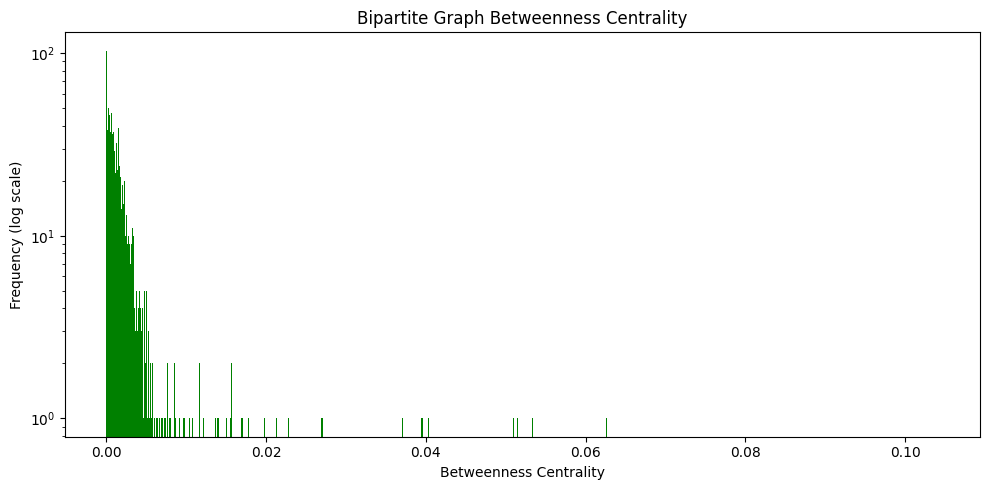
\includegraphics[width=1\columnwidth]{bet_entire.png}
    \caption{Betweenness Centrality of the entire network}
    \label{fig:bet_entire}
\end{figure}

\begin{figure}[H]
    \centering
    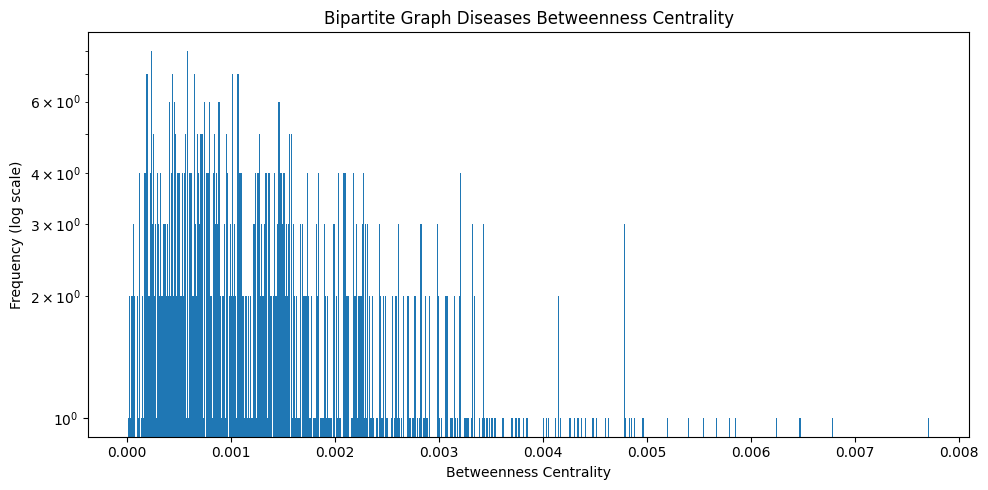
\includegraphics[width=1\columnwidth]{bet_diseases.png}
    \caption{Betweenness Centrality of the diseases}
    \label{fig:bet_diseases}
\end{figure}

\begin{figure}[H]
    \centering
    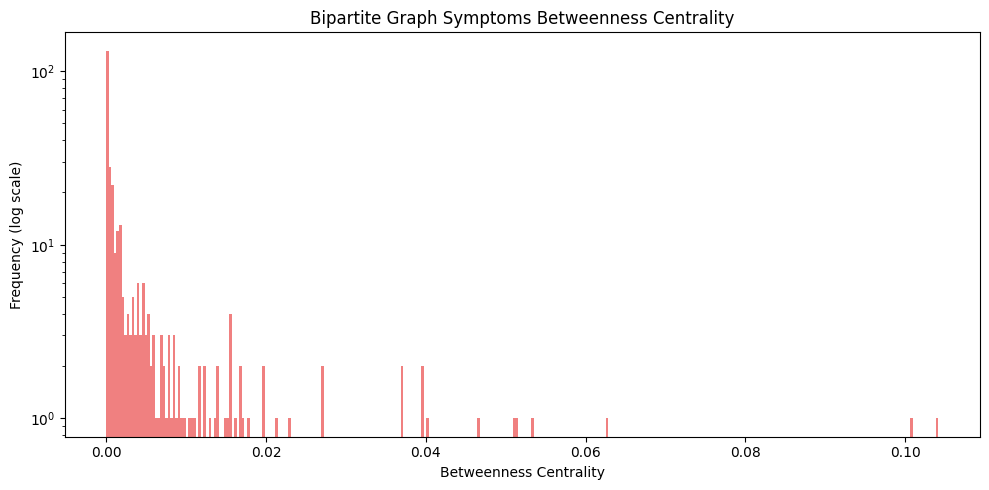
\includegraphics[width=1\columnwidth]{bet_symptoms.png}
    \caption{Betweenness Centrality of the symptoms}
    \label{fig:bet_symptoms}
\end{figure}

\begin{figure}[H]
   \centering
   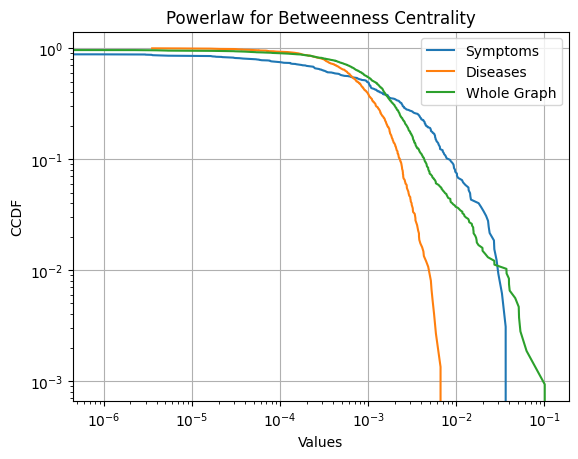
\includegraphics[width=1\columnwidth]{bet_all.png}
   \caption{Betweenness Centrality CDFs}
   \label{fig:bet_all}
\end{figure}

\begin{figure}[H]
    \centering
    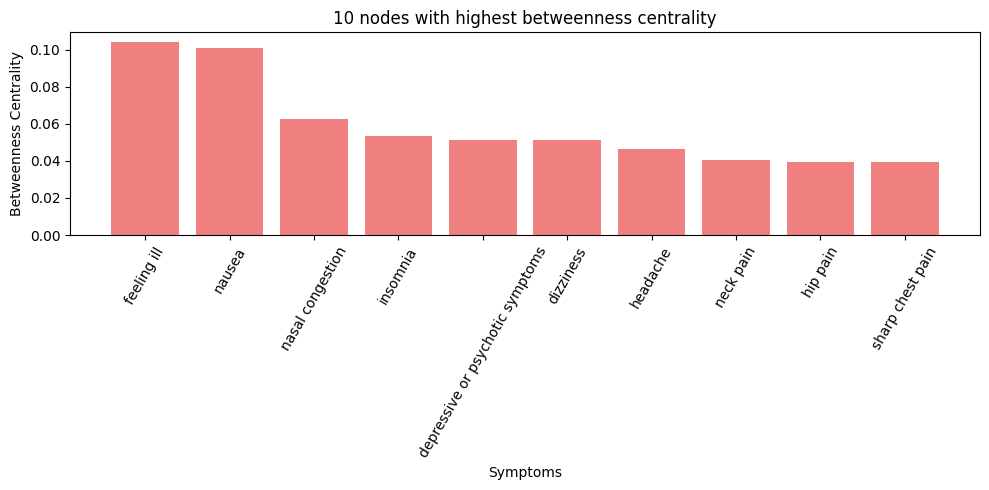
\includegraphics[width=1\columnwidth]{bet_top.png}
    \caption{Top 10 nodes with the highest betweenness centrality}
    \label{fig:bet_top}
\end{figure}

% END: betweenness centrality

\subsection{Communities}
% BEGIN: communities
The detection of communities in a network can be useful both for the interpretation of the network itself and for the ML model prediction Enhancing.
As regard the network interpretation it is worth to underline that a community of symptoms identifies a set of symptoms that are 
often co-occurring within the same diseases, while a community of diseases identifies a set of diseases that are often co-occurring within the same symptoms.
The size of the different communities is reported in Figure \ref{fig:com_sizes_all}.

Given a symptoms community could be of clinical interest to understand which are the diseases that are most often associated with the symptoms of the community.
This information is depicted in (Figures \ref{fig:com1_symptoms}, \ref{fig:com2_symptoms} and \ref{fig:com3_symptoms}). 
As an interpretation example we can look at the community 1 of symptoms (Figure \ref{fig:com1_symptoms}). In this case we can say that 'herniated disk' is the 
third most pointed disease by the symptoms of the community. It is pointed by 12 symptoms each one pointing on average 3 diseases.

The same kind of study can be done for the communities of diseases. In this case the results are shown in Figures \ref{fig:com1_diseases}, 
\ref{fig:com2_diseases} and \ref{fig:com3_diseases}. This kind of information could be useful to profile the diseases and understanding the significance
of each symptom. For example, looking at community 1 of diseases (Figure \ref{fig:com1_diseases}), the 'sharp abdominal pain' symptom is present in almost 
half of the diseases of the community. This means that this symptom is very generic and it is not very useful to discriminate between the diseases of the community.

Switching now the the creation of features for the Ml model, we created two kinds of features: 
\begin{itemize}
    \item \textbf{Community Count}: taking a symptoms one hot vector, we count how many symptoms of the vector are in each community. The new features vector 
    has a length equal to the number of communities and a value equal to the number of symptoms of the original vector that are in the community.
    \item \textbf{Community Size}: taking a symptoms one hot vector, we replace each symptom with the size of the community of the symptom.
\end{itemize}



\begin{figure}[H]
    \centering
    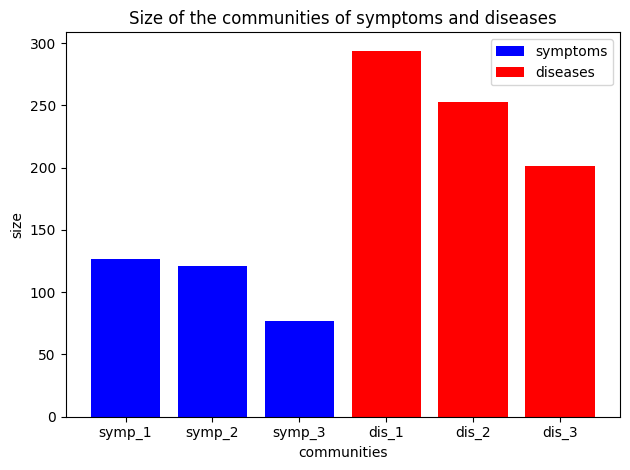
\includegraphics[width=1\columnwidth]{com_sizes_all.png}
    \caption{Sizes of the communities of symptoms and diseases}
    \label{fig:com_sizes_all}
\end{figure}

\begin{figure}[H]
    \centering
    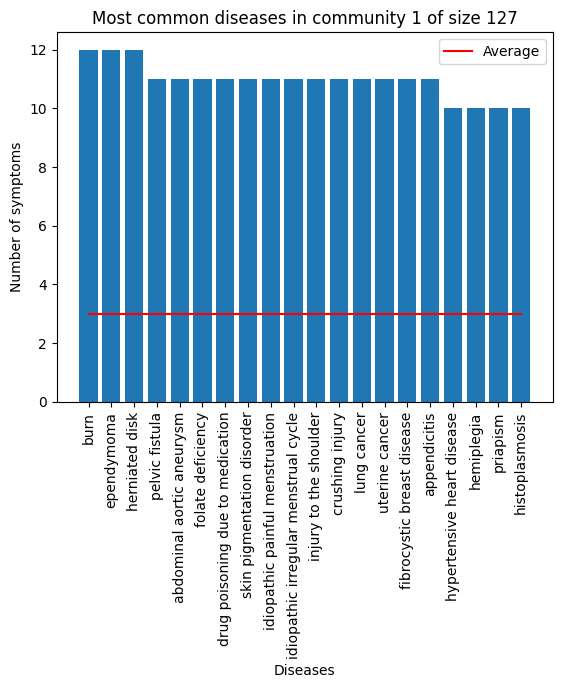
\includegraphics[width=1\columnwidth]{com1_symptoms.png}
    \caption{Community 1 of symptoms}
    \label{fig:com1_symptoms}
\end{figure}

\begin{figure}[H]
    \centering
    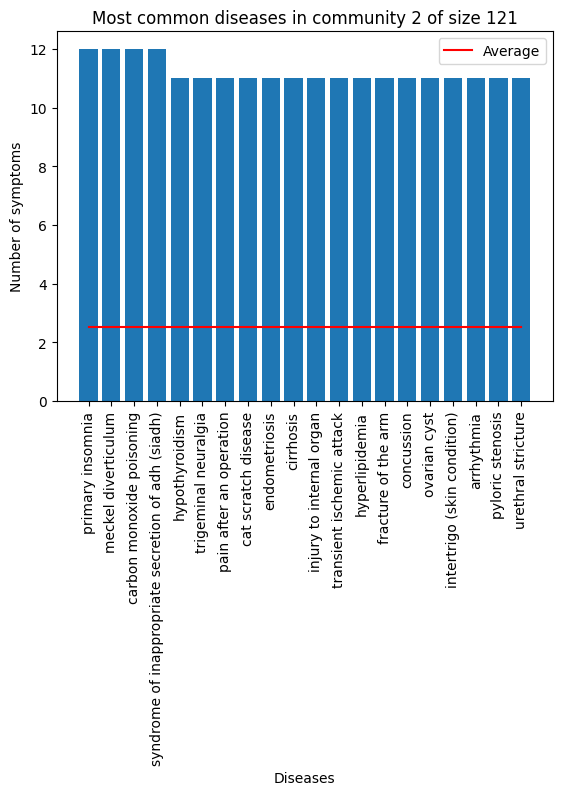
\includegraphics[width=1\columnwidth]{com2_symptoms.png}
    \caption{Community 2 of symptoms}
    \label{fig:com2_symptoms}
\end{figure}

\begin{figure}[H]
    \centering
    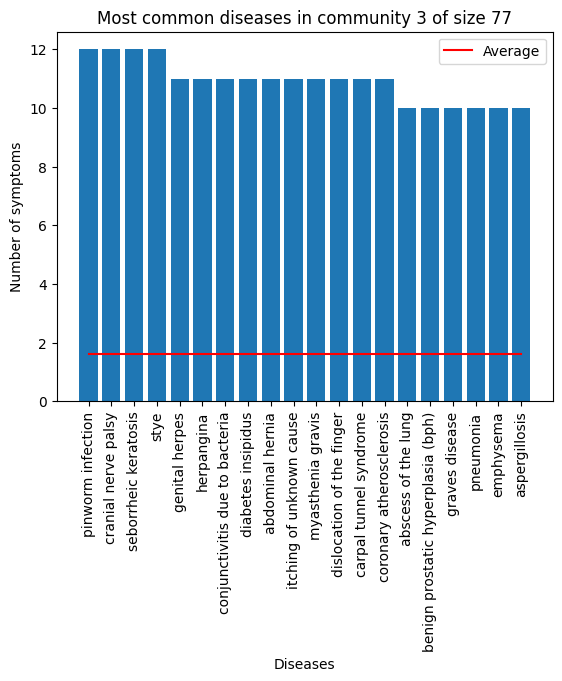
\includegraphics[width=1\columnwidth]{com3_symptoms.png}
    \caption{Community 3 of symptoms}
    \label{fig:com3_symptoms}
\end{figure}

\begin{figure}[H]
    \centering
    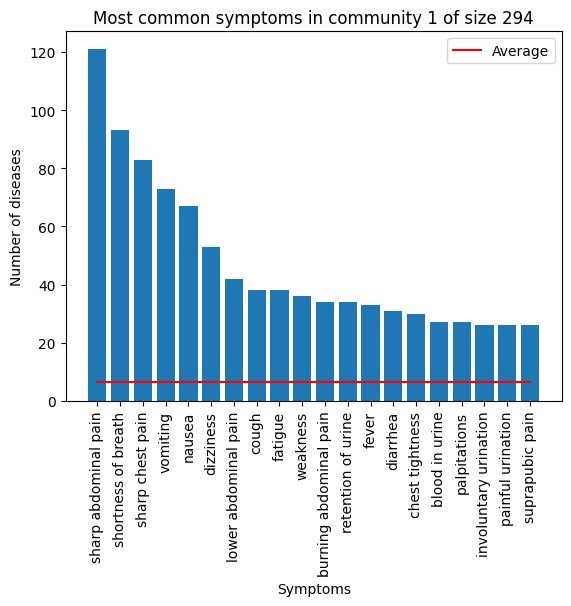
\includegraphics[width=1\columnwidth]{com1_diseases.png}
    \caption{Community 1 of diseases}
    \label{fig:com1_diseases}
\end{figure}

\begin{figure}[H]
    \centering
    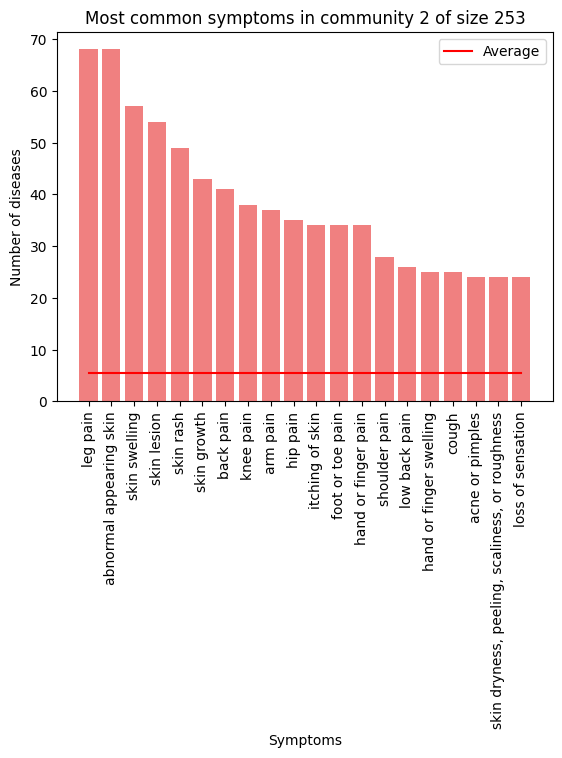
\includegraphics[width=1\columnwidth]{com2_diseases.png}
    \caption{Community 2 of diseases}
    \label{fig:com2_diseases}
\end{figure}

\begin{figure}[H]
    \centering
    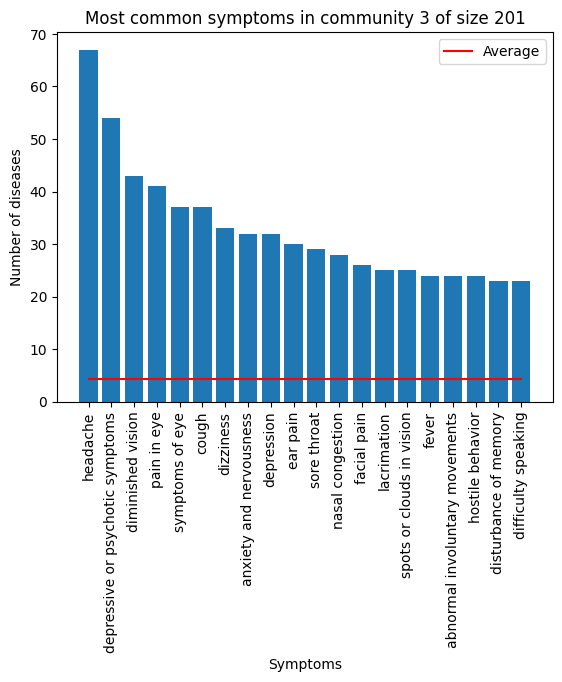
\includegraphics[width=1\columnwidth]{com3_diseases.png}
    \caption{Community 3 of diseases}
    \label{fig:com3_diseases}
\end{figure}



% END: communities


